\documentclass[12pt, twoside]{article}
\documentclass[12pt, twoside]{article}
\usepackage[letterpaper, margin=1in, headsep=0.2in]{geometry}
\setlength{\headheight}{0.6in}
%\usepackage[english]{babel}
\usepackage[utf8]{inputenc}
\usepackage{microtype}
\usepackage{amsmath}
\usepackage{amssymb}
%\usepackage{amsfonts}
\usepackage{siunitx} %units in math. eg 20\milli\meter
\usepackage{yhmath} % for arcs, overparenth command
\usepackage{tikz} %graphics
\usetikzlibrary{quotes, angles}
\usepackage{graphicx} %consider setting \graphicspath{{images/}}
\usepackage{parskip} %no paragraph indent
\usepackage{enumitem}
\usepackage{multicol}
\usepackage{venndiagram}

\usepackage{fancyhdr}
\pagestyle{fancy}
\fancyhf{}
\renewcommand{\headrulewidth}{0pt} % disable the underline of the header
\raggedbottom
\hfuzz=2mm %suppresses overfull box warnings

\usepackage{hyperref}
\usepackage{float}

\title{Algebra 2}
\author{Chris Huson}
\date{November 2024}

\fancyhead[LE]{\thepage}
\fancyhead[RO]{\thepage \\ First and last name: \hspace{2.5cm} \,\\ Section: \hspace{2.5cm} \,}
\fancyhead[LO]{BECA / Huson / Algebra 2: Polynomials \\* 6 November 2024}

\begin{document}

\subsubsection*{Quiz: Rational functions (optional plus standards)}
\begin{enumerate}[itemsep=0.5cm]

    \item The expression $\displaystyle \frac{x^4 - 5x^2 + 4x + 14}{x+2}$ is equivalent to
    \begin{enumerate}
        \item $\displaystyle x^3 - 2x^2 - x + 6 - \frac{2}{x + 2}$
        \item $\displaystyle x^3 - 5x + 4 - \frac{14}{x + 2}$
        \item $\displaystyle x^3 + 2x^2 - x + 2 + \frac{18}{x + 2}$
        \item $\displaystyle x^3 + 2x^2 - 9x + 22 - \frac{30}{x + 2}$
    \end{enumerate}
    
    \item What is the solution set of the equation \(\displaystyle \frac{x+2}{x} + \frac{x}{3} = \frac{2x^2+6}{3x}\)?
    \begin{enumerate}
        \item \(\{-3\}\)
        \item \(\{-3, 0\}\)
        \item \(\{3\}\)
        \item \(\{0, 3\}\)
    \end{enumerate}
    
    \item Which equation represents a polynomial identity? %January 2023 Regents
    \begin{enumerate}
        \item \(x^3 + y^3 = (x + y)^3\)
        \item \(x^3 + y^3 = (x + y)(x^2 - xy + y^2)\)
        \item \(x^3 + y^3 = (x + y)(x^2 - xy - y^2)\)
        \item \(x^3 + y^3 = (x - y)(x^2 + xy + y^2)\)
    \end{enumerate}
    
\newpage 
\item Use polynomial long division \hfill (A.APR.6 Rewrite rational expressions) \\[0.5cm]
 to find an expression of the form $ax^2 + bx +c +\frac{d}{x+e}$ with $a,b,c,d,e$ integers that is equivalent to $\displaystyle \frac{x^3 + 9x^2 - 5x - 90}{x + 4}
$ for $x \neq -4$.
\vspace{10cm}

\item Solve for $x$. \hfill (A.REI.4 Solve quadratic equations algebraically)
$$\frac{4}{x+2} = \frac{x-3}{x}$$ \vspace{4cm}

\newpage 
\subsubsection*{A2-APR.1 Perform operations with polynomials}
\item Find the sum in standard form $(4x^4+5x^3+3x^2-4) + (x^4-2x^3-2x^2-x+1)$. \vspace{3cm}

\item Which expression is equivalent to $(x + 2)^2 - 5(x + 2) + 6$?
\begin{enumerate}
    \item $x(x + 1)$
    \item $(x - 3)(x + 2)$
    \item $(x - 4)(x + 3)$
    \item $(x - 6)(x + 1)$
\end{enumerate}

\newpage
\item Write the expression $A(x) \cdot B(x) - 3C(x)$ as a polynomial in standard form. %2 points January 2023 Regents
\begin{align*}
    A(x) &= x^3 + 2x - 1 \\
    B(x) &= x^2 + 7 \\
    C(x) &= x^4 - 5x
\end{align*}

\item Stone Manufacturing has developed a cost model, $C(x) = 0.18x^3 + 0.02x^2 + 4x + 180$, where $x$ is the number of sprockets sold, in thousands. The sale price can be modeled by $S(x) = 95.4 - 6x$ and the company’s revenue by $R(x) = x \cdot S(x)$. The company profits, $R(x) - C(x)$, could be modeled by %August 2023 Regents
\begin{enumerate}
    \item $0.18x^3 + 6.02x^2 + 91.4x + 180$
    \item $0.18x^3 - 5.98x^2 - 91.4x + 180$
    \item $-0.18x^3 - 6.02x^2 + 91.4x - 180$
    \item $0.18x^3 + 5.98x^2 + 99.4x + 180$
\end{enumerate}

\newpage
\item Given the rational function $\displaystyle r(x)= \frac{x+3}{x-2}-3$. \hfill (F.IF.7d Graph rational functions)
    \begin{enumerate}[itemsep=0.25cm]
        \item Sketch a graph of the function.
        \item Mark the vertical asymptote as dotted line and label it with its equation.
        \item Explain why the asymptote is located there.
    \end{enumerate}
    \begin{center}
    \begin{tikzpicture}[xscale=0.7, yscale=0.7]
        \draw [thick, ->] (-8.2,0) -- (8.5,0) node [above] {$x$};
        \draw [thick, ->] (0,-8.2)--(0,8.5) node [right] {$y$};
        \foreach \x in {-8,-6,-4,-2,2,4,6,8} \draw (\x cm,5pt)--(\x cm,-5pt) node at (\x,-0.5){\x};
        \foreach \y in {-8,-6,-4,-2,2,4,6,8} \draw (5pt,\y cm)--(-5pt,\y cm) node at (-0.5,\y){\y};
    \end{tikzpicture}
    \end{center}
    
\newpage
\subsubsection*{A2-F.IF.7c Graph polynomials, identify zeros, end behavior}
\item The polynomial $f(x)$ and linear function $g(x)$ are graphed below. 
\begin{multicols}{2}
    \begin{enumerate}[itemsep=0.6cm]
        \item What is the degree of $f(x)$?
        \item Is the leading coefficient of $f(x)$ positive, negative, or zero?
        \item If the polynomial $f(x)$ is written as the product of linear factors, what factor would be squared?
        \item Write down the three solutions to $f(x)=g(x)$ as ordered pairs.
    \end{enumerate} \vspace{1cm} \;

    \columnbreak

    \begin{tikzpicture}[xscale=0.7, yscale=0.7]
        \draw[lightgray,very thin] (-4,-2) grid (4,10);
        \draw [thick, ->] (-4.2,0) -- (4.4,0) node [above] {$x$};
        \draw [thick, ->] (0,-2.2)--(0,10.5) node [right] {$y$};
        \foreach \x in {-4,4} \draw (\x cm,5pt)--(\x cm,-5pt)node[below]{$\x$};
        \foreach \y in {-1,5,10} \draw (5pt,\y cm)--(-5pt,\y cm)node[left]{$\y$};
        \draw [thick, <->,smooth,samples=20,domain=3.15:-3.6] plot(\x,{-0.5*(\x-3)*(\x+2)^2})node[right]{\footnotesize $f(x)$};
        \draw [thick, <->,smooth,samples=20,domain=3.7:-3.7] plot(\x,{-0.5*(\x)+1.5})node[below left]{\footnotesize $g(x)$};
    \end{tikzpicture}
\end{multicols}

\subsubsection*{A2-F.BF.2 Write arithmetic and geometric sequences with recursive formulas}
\item Write a recursive definition of the sequence $a_1 = 2$, $a_2 = 6$, $a_3 = 18$, $a_4 = 54, \ldots$ \vspace{2cm}

\end{enumerate}
\end{document}